\documentclass[12pt,a4paper]{article}

% Packages
\usepackage[utf8]{inputenc}
\usepackage{amsmath}
\usepackage{amsfonts}
\usepackage{amssymb}
\usepackage{graphicx}
\usepackage{hyperref}
\usepackage{algorithm}
\usepackage{algpseudocode}
\usepackage{booktabs}
\usepackage{listings}
\usepackage{enumerate}
\usepackage{pythontex}
\usepackage{lstmisc}
\usepackage{subcaption}


\usepackage{tikz}
\usepackage{xcolor}
\usepackage{siunitx}
\usepackage{float}
\usepackage{cleveref}

% Document settings
\title{Sudoku Forschungsprojekt Dokumentation}
\author{Bastian Fischer, Samuel Jaschke, Hannes Träger, Paul Volk}
\date{\today}

\begin{document}

\maketitle

\begin{abstract}
\end{abstract}

\section{Einführung}
\subsection{Hintergrund}

\subsection{Forschungsziele}
Es werden folgende Forschungsziele behandelt:
\begin{itemize}
    \item  
\end{itemize}

\section{Theoretische Überlegungen}

\subsection{Problem Formulierung}

\subsection{Minimale Anzahl Hinweise}
Die minimale Anzahl für ein eindeutig lösbares $9 \times 9$ Sudoku sind 17 Hinweise~\cite{DBLP:journals/corr/abs-1201-0749}.
Für $4 \times 4$ und $6 \times 6$ Sudokus haben wir alles Anordnungen an Hinweisen selbst getestet.
Für $4 \times 4$ Sudokus sind es 4 Hinweise und für $6 \times 6$ Sudokus sind es %TODO
Hinweise.
%TODO jeweils ein Sudoku einfügen


\subsection{Symmetrien}
Ein Sudoku besteht aus 3 horizontalen und 3 vertikalen Bändern. Die Bänder bestehen jeweils aus 3 Zeilen beziehungsweise 3 Spalten. \\
Die Tupel (1, 2, 3),(4, 5, 6),(7, 8, 9) beschreiben die Zeilen oder Spalten der jeweiligen Bänder. \\
Mit dem Wissen über die Bänder können wir die Symmetrien eines Sudokus formulieren~\cite{russell2006mathematics}: \\
\begin{itemize}
    \item Permutation der 9 Ziffern
    \item Permutation der 3 horizontalen Bänder
    \item Permutation der 3 vertikalen Bänder
    \item Permutation der Zeilen innerhalb eines horizontalen Bandes
    \item Permutation der Spalten innerhalb eines vertikalen Bandes
    \item Spiegelung und Rotation
\end{itemize}
Insgesamt gibt es in etwa 6,7 Trilliarden verschiedene valide Sudokus \cite{felgenhauer2006mathematics}. Unter Berücksichtigung der Symmetrien
gibt es ungefähr 5,5 Milliarden verschiedene valide Sudokus\cite{russell2006mathematics}. \\


\subsection{Anzahl Hinweise pro Band}

\begin{figure}[H]
    \centering
    \begin{minipage}{0.48\textwidth}
        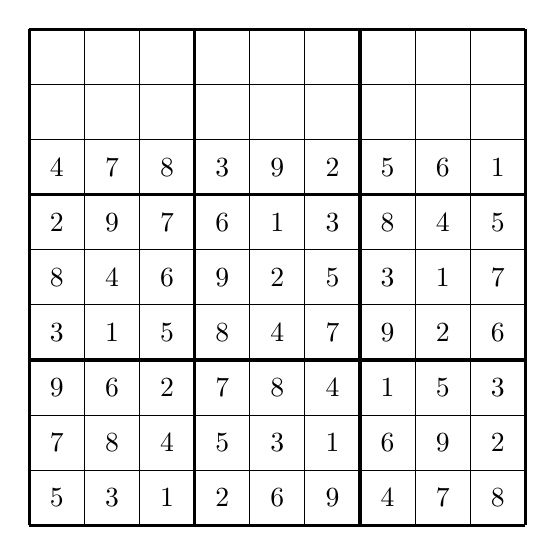
\begin{tikzpicture}
            % Zellgröße
            \def\s{0.7cm}

            % Sudoku-Lösung (kann beliebig angepasst werden)
            \def\sudoku{
                    {, , , , , , , , },
                    {, , , , , , , , },
                    {4, 7, 8, 3, 9, 2, 5, 6, 1},
                    {2, 9, 7, 6, 1, 3, 8, 4, 5},
                    {8, 4, 6, 9, 2, 5, 3, 1, 7},
                    {3, 1, 5, 8, 4, 7, 9, 2, 6},
                    {9, 6, 2, 7, 8, 4, 1, 5, 3},
                    {7, 8, 4, 5, 3, 1, 6, 9, 2},
                    {5, 3, 1, 2, 6, 9, 4, 7, 8},
            }

            % Rasterlinien
            \foreach \x in {0,1,...,9} {
                \draw[thin] (\x*\s, 0) -- (\x*\s, 9*\s);
                \draw[thin] (0, \x*\s) -- (9*\s, \x*\s);
            }
            \foreach \x in {0,3,6,9} {
                \draw[very thick] (\x*\s, 0) -- (\x*\s, 9*\s);
                \draw[very thick] (0, \x*\s) -- (9*\s, \x*\s);
            }




            % Zahlen eintragen
            \foreach \row [count=\i from 0] in \sudoku {
                \foreach \num [count=\j from 0] in \row {
                % Y-Koordinate: Startet oben bei 8.5 und geht pro Zeile 1 runter
                    \node at (\j*\s + 0.5*\s, 8.5*\s - \i*\s) {\num};
                }
            }
        \end{tikzpicture}
    \end{minipage}
    \hfill
    \begin{minipage}{0.48\textwidth}
        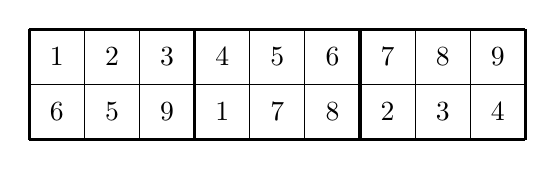
\begin{tikzpicture}[baseline]
            % Zellgröße
            \def\s{0.7cm}

            % Werte für das 2x9 Gitter
            \def\zweizeilen{
                    {1, 2, 3, 4, 5, 6, 7, 8, 9},
                    {6, 5, 9, 1, 7, 8, 2, 3, 4},
            }

            % Rasterlinien
            \foreach \x in {0,1,...,9} {
                \draw[thin] (\x*\s, 0) -- (\x*\s, 2*\s);
            }
            \foreach \y in {0,1,2} {
                \draw[thin] (0, \y*\s) -- (9*\s, \y*\s);
            }

            % Dickere Linien wie bei Sudoku
            \foreach \x in {0,3,6,9} {
                \draw[very thick] (\x*\s, 0) -- (\x*\s, 2*\s);
            }
            \draw[very thick] (0, 0) -- (9*\s, 0);
            \draw[very thick] (0, 2*\s) -- (9*\s, 2*\s);

            % Zahlen eintragen
            \foreach \row [count=\i from 0] in \zweizeilen {
                \foreach \num [count=\j from 0] in \row {
                    \node at (\j*\s + 0.5*\s, 1.5*\s - \i*\s) {\num};
                }
            }
        \end{tikzpicture}
        \\
        \\

        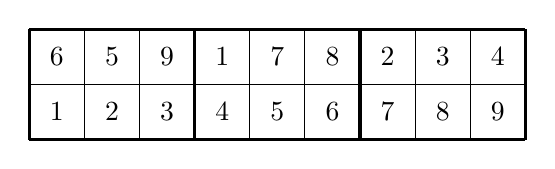
\begin{tikzpicture}[baseline]
            % Zellgröße
            \def\s{0.7cm}

            % Werte für das 2x9 Gitter
            \def\zweizeilen{
                    {6, 5, 9, 1, 7, 8, 2, 3, 4},
                    {1, 2, 3, 4, 5, 6, 7, 8, 9},
            }

            % Rasterlinien
            \foreach \x in {0,1,...,9} {
                \draw[thin] (\x*\s, 0) -- (\x*\s, 2*\s);
            }
            \foreach \y in {0,1,2} {
                \draw[thin] (0, \y*\s) -- (9*\s, \y*\s);
            }

            % Dickere Linien wie bei Sudoku
            \foreach \x in {0,3,6,9} {
                \draw[very thick] (\x*\s, 0) -- (\x*\s, 2*\s);
            }
            \draw[very thick] (0, 0) -- (9*\s, 0);
            \draw[very thick] (0, 2*\s) -- (9*\s, 2*\s);

            % Zahlen eintragen
            \foreach \row [count=\i from 0] in \zweizeilen {
                \foreach \num [count=\j from 0] in \row {
                    \node at (\j*\s + 0.5*\s, 1.5*\s - \i*\s) {\num};
                }
            }
        \end{tikzpicture}
    \end{minipage}
    \caption{Beispiel für Zeilenvertauschung}
    \label{fig:row_constraints}
\end{figure}

In einem partiellen Sudoku darf es in einem horizontalen Band keine zwei Zeilen ohne Hinweise geben.
In \cref{fig:row_constraints} kann man sehen das es ansonsten mehrere Lösungen gibt.
Alle Hinweise bis auf zwei komplette Zeilen sind gegeben und es gibt trotzdem zwei Lösungen, welche man rechts sehen kann.
Äquivalent dazu dürfen in einem vertikalen Band keine zwei Spalten ohne Hinweise sein.
Übersetzt man dies auf allgemeine Sudoku-Größen,
muss in einem Band der Breite beziehungsweise Höhe $n$ mindestens $n-1$ Spalten beziehungsweise Zeilen mit Hinweisen gegeben sein.


\subsection{Unterquadrate}

\begin{figure}[H]
    \centering
    \begin{minipage}{0.48\textwidth}
        \begin{tikzpicture}
            \begin{tikzpicture}
                % Zellgröße
                \def\s{0.7cm}

                % Sudoku-Lösung (kann beliebig angepasst werden)
                \def\sudoku{
                        {1, 2, 3, 4, 5, 6, 7, 8, 9},
                        {6, 5, 9, 1, 7, 8, 2, 3, 4},
                        {4, 7, 8, 3, 9, 2, 5, 6, 1},
                        {2, 9, 7, 6, 1, 3, 8, 4, 5},
                        {8, 4, 6, 9, 2, 5, 3, 1, 7},
                        {3, 1, 5, 8, 4, 7, 9, 2, 6},
                        {9, 6, 2, 7, 8, 4, 1, 5, 3},
                        {7, 8, 4, 5, 3, 1, 6, 9, 2},
                        {5, 3, 1, 2, 6, 9, 4, 7, 8},
                }

                \fill[green!30] (5*\s, 5*\s) rectangle (6*\s, 6*\s);
                \fill[green!30] (4*\s, 5*\s) rectangle (5*\s, 6*\s);

                \fill[green!30] (5*\s, 1*\s) rectangle (6*\s, 2*\s);
                \fill[green!30] (4*\s, 1*\s) rectangle (5*\s, 2*\s);

                % Rasterlinien
                \foreach \x in {0,1,...,9} {
                    \draw[thin] (\x*\s, 0) -- (\x*\s, 9*\s);
                    \draw[thin] (0, \x*\s) -- (9*\s, \x*\s);
                }
                \foreach \x in {0,3,6,9} {
                    \draw[very thick] (\x*\s, 0) -- (\x*\s, 9*\s);
                    \draw[very thick] (0, \x*\s) -- (9*\s, \x*\s);
                }




                % Zahlen eintragen
                \foreach \row [count=\i from 0] in \sudoku {
                    \foreach \num [count=\j from 0] in \row {
                    % Y-Koordinate: Startet oben bei 8.5 und geht pro Zeile 1 runter
                        \node at (\j*\s + 0.5*\s, 8.5*\s - \i*\s) {\num};
                    }
                }
            \end{tikzpicture}
        \end{tikzpicture}
    \end{minipage}
    \hfill
    \begin{minipage}{0.48\textwidth}
        \begin{tikzpicture}
            \begin{tikzpicture}
                % Zellgröße
                \def\s{0.7cm}

                % Sudoku-Lösung (kann beliebig angepasst werden)
                \def\sudoku{
                        {1, 2, 3, 4, 5, 6, 7, 8, 9},
                        {6, 5, 9, 1, 7, 8, 2, 3, 4},
                        {4, 7, 8, 3, 9, 2, 5, 6, 1},
                        {2, 9, 7, 6, 3, 1, 8, 4, 5},
                        {8, 4, 6, 9, 2, 5, 3, 1, 7},
                        {3, 1, 5, 8, 4, 7, 9, 2, 6},
                        {9, 6, 2, 7, 8, 4, 1, 5, 3},
                        {7, 8, 4, 5, 1, 3, 6, 9, 2},
                        {5, 3, 1, 2, 6, 9, 4, 7, 8},
                }

                \fill[green!30] (5*\s, 5*\s) rectangle (6*\s, 6*\s);
                \fill[green!30] (4*\s, 5*\s) rectangle (5*\s, 6*\s);

                \fill[green!30] (5*\s, 1*\s) rectangle (6*\s, 2*\s);
                \fill[green!30] (4*\s, 1*\s) rectangle (5*\s, 2*\s);

                % Rasterlinien
                \foreach \x in {0,1,...,9} {
                    \draw[thin] (\x*\s, 0) -- (\x*\s, 9*\s);
                    \draw[thin] (0, \x*\s) -- (9*\s, \x*\s);
                }
                \foreach \x in {0,3,6,9} {
                    \draw[very thick] (\x*\s, 0) -- (\x*\s, 9*\s);
                    \draw[very thick] (0, \x*\s) -- (9*\s, \x*\s);
                }




                % Zahlen eintragen
                \foreach \row [count=\i from 0] in \sudoku {
                    \foreach \num [count=\j from 0] in \row {
                    % Y-Koordinate: Startet oben bei 8.5 und geht pro Zeile 1 runter
                        \node at (\j*\s + 0.5*\s, 8.5*\s - \i*\s) {\num};
                    }
                }
            \end{tikzpicture}
        \end{tikzpicture}
    \end{minipage}
    \caption{Gemeinsame Beschriftung für beide Sudoku-Gitter}
    \label{fig:gemeinsames_sudoku}
\end{figure}

Innerhalb von vollständig ausgefüllten Sudokus kann es Unterquadrate geben.
Ein Beispiel für ein solches Unterquadrat ist in \cref{fig:gemeinsames_sudoku} gegeben.
Ein Unterquadrat besteht aus vier Zellen in denen zwei Ziffern jeweils doppelt vorkommen.
Je zwei Zellen sind dabei in der gleichen Spalte beziehungsweise in der gleichen Zeile.
Entweder beide Zeilen oder beide Spalten sind im gleichen Band.
Durch die Anordnung der Zellen ist es möglich, ein weiteres gültiges Sudoku zu generieren, nur durch Permutieren der beiden Ziffern im Unterquadrat.
Das heißt, um ein eindeutig lösbares partielles Sudoku aus diesem voll ausgefüllten Sudoku zu erhalten,
muss mindestens eine der Zellen des Unterquadrats Teil des partiellen Sudokus sein.
Einige vollständige Sudokus haben sehr viele Unterquadrate und sind dementsprechend weniger gut geeignet,
um daraus ein partielles Sudoku zu generieren.
Um unsere Liste an vollständigen Sudokus für die Suche zu verbessern, generieren wir nur Sudokus, die keine Unterquadrate enthalten.

\section{Erzeugung der partiellen Sudokus}

\input{Sections/Erzeugung Lösung}

\begin{table}[h!]
    \centering
    \begin{tabular}{|c|c|c|c|}
        \hline
        \textbf{Anzahl Hinweise} & \textbf{Anzahl true} & \textbf{Anzahl total} & \textbf{Wahrscheinlichkeit} \\
        \hline
        21 & 0     & 3     & 0.00\% \\
        22 & 4     & 147   & 2.72\% \\
        23 & 786   & 1829  & 42.97\% \\
        24 & 10883 & 11879 & 91.62\% \\
        25 & 30508 & 30638 & 99.58\% \\
        26 & 33783 & 33786 & 99.99\% \\
        27 & 16948 & 16948 & 100.00\% \\
        28 & 4235  & 4235  & 100.00\% \\
        29 & 513   & 513   & 100.00\% \\
        30 & 21    & 21    & 100.00\% \\
        31 & 1     & 1     & 100.00\% \\
        \hline
    \end{tabular}
    \caption{Übersicht: Anzahl Hinweise, Anzahl true, Anzahl total und Wahrscheinlichkeit (in Prozent) pro Wert}
\end{table}

\begin{figure}[h!]
    \centering
    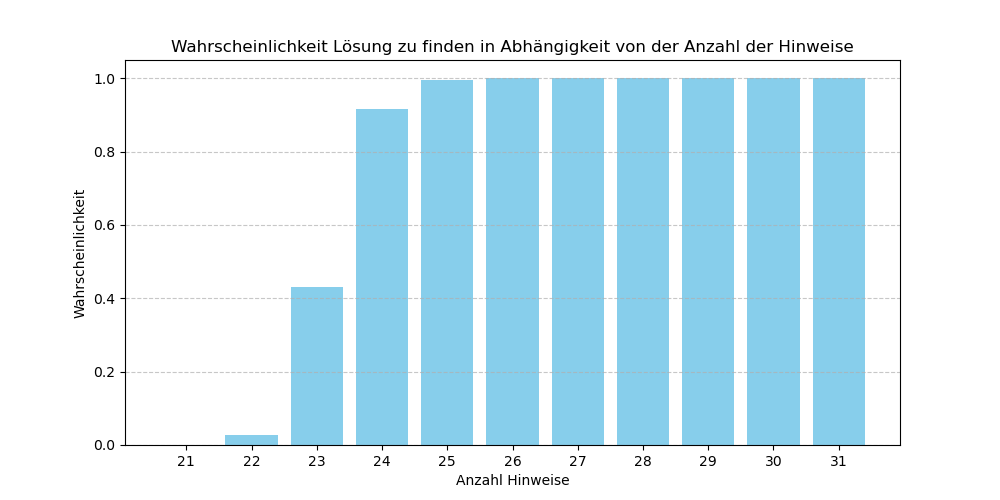
\includegraphics[width=0.8\textwidth]{Pictures/wahrscheinlichkeiten}
    \caption{Wahrscheinlichkeit, dass ein Sudoku mit einer bestimmten Anzahl an Hinweisen eindeutig lösbar ist}
    \label{fig:wahrscheinlichkeiten}

\end{figure}

\begin{figure}[h!]
    \centering
    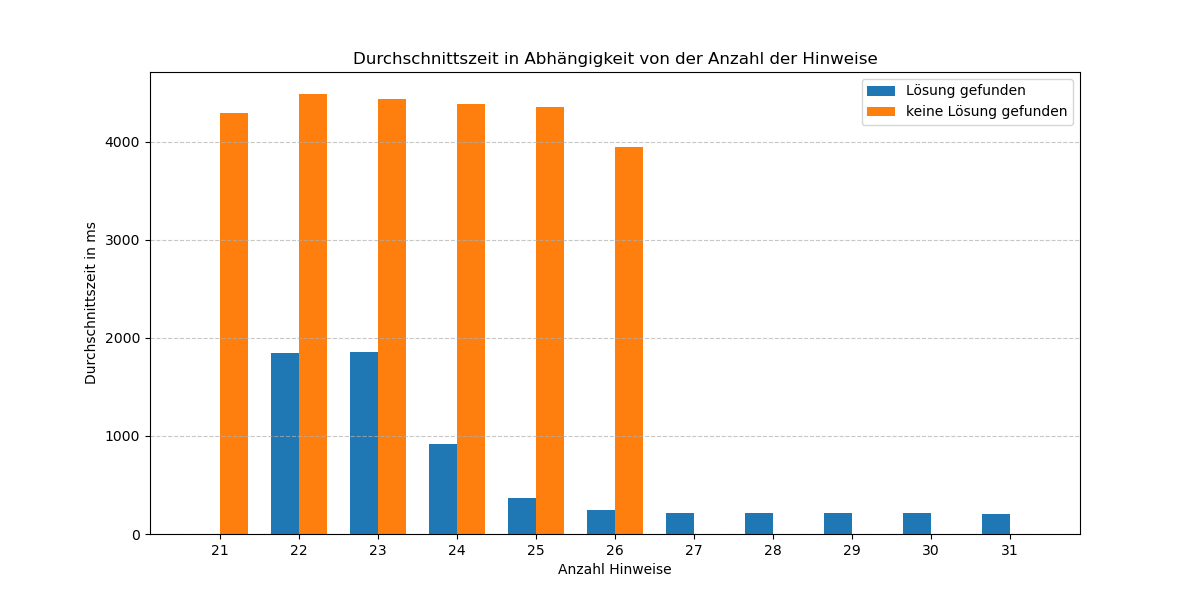
\includegraphics[width=0.8\textwidth]{Pictures/zeiten}
    \caption{Wahrscheinlichkeit, dass ein Sudoku mit einer bestimmten Anzahl an Hinweisen eindeutig lösbar ist}
    \label{fig:zeiten}
\end{figure}

\section{ab hier steht der nicht schöne von Basti und Sammy generierte Code}
\subsection{Algorithmen}
\subsubsection{Generierungsalgorithmen}
Um zu überprüfen ob ein Sudoku eindeutig ist, nutzen wir folgenden Algorithmus~\ref{alg:eindeutig}. 
Wenn also durch die Anwendung des Grids auf die Lösungen ein eindeutig lösbares Sudoku entsteht können wir dieses dem Nutzer zurückgeben.
Im Algorithmus~\ref{alg:generierung} wird dargestellt, wie wir hierbei vorgehen.

\begin{algorithm}
    \caption{Sudoku eindeutig lösbar}
    \label{alg:eindeutig}
    \begin{algorithmic}[1]
        \Require $G$ ist ein leeres oder teilweise ausgefülltes $9 \times 9$ Sudoku-Gitter.
        \Require $Solver$ ist eine SAT-Solver mit den entsprechenden Sudoku Klauseln.
        \Ensure Es wird \textbf{true} und die Lösung zurück gegeben wenn das Sudoku eindeutig lösbar ist und \textbf{false} wenn nicht.
        \Function{Eindeutig}{$G, Solver$}
            \State Let $solvable, solution \gets \Call{Solver.solveSudoku}{G}$
            \If{solvable}
                \State $\Call{Solver.prohibitSolution}{solution}$
                \State Let $unique, uniqueSolution \gets \Call{Solver.solveSudoku}{G}$
                \State \Return (unique, $uniqueSolution$)
            \Else
                \State \Return \textbf{false}
            \EndIf
        \EndFunction
    \end{algorithmic}
\end{algorithm}


\begin{algorithm}
    \caption{Sudoku Generierung}
    \label{alg:generierung}
    \begin{algorithmic}[1]
        \Require $G$ ist ein Sudoku-Gitter mit Einsen an markierten und Nullen and unmarkierten Stellen.
        \Require $M$ Menge an vollständigen Sudokus, die wir zur Generierung nutzen.
        \Function{generateSudoku}{$G, M$}
            \State Let $solver \gets \Call{Solver}{G.size}$
            \For{$m \in M$}
                \State Let $transformed \gets G \cdot m$ \Comment{Stellenweise Multiplikation}
                \State Let $unique, solution \gets \Call{Eindeutig}{transformed, solver}$
                \If{$unique$}
                    \State \Return $solution$
                \EndIf
            \EndFor
            
        \EndFunction
    \end{algorithmic}
\end{algorithm}

Beim Generieren wurden zwei verschiedene Möglichkeiten verglichen, einmal die Generierung ohne und einmal mit Threads. 
Das Generieren zu parallelisieren scheint sinnvoll, da es keine großen Abhängigkeiten voneinander gibt.
Die Implementierung mit Threads ist im Grunde die gleiche wie ohne, nur, dass hier die Menge $M$ in die Anzahl von Threads viele disjunktive Teilmengen geteilt wird.
Anschließend wird auf jeder Thread auf einer dieser Teilmengen gestartet. Sobald eine Lösung gefunden wird, werden die anderen Threads unterbrochen.

\subsubsection{Lösungsalgorithmen}
\input{Sections/Lösungsalgorithmen.tex}

\subsection{Implementierung}
\subsection{Kommunikation per POST-Anfrage}

Die Kommunikation zwischen Frontend und Backend erfolgt über POST-Anfragen. Das Frontend sendet dabei Daten im JSON-Format an einen definierten API-Endpunkt des Backends.

\subsection{Frontend-Seite}

Das Frontend erstellt ein JSON-Objekt mit den benötigten Daten und schickt es per POST an das Backend. Beispiel mit JavaScript:

\begin{verbatim}
fetch('/api/endpoint', {
  method: 'POST',
  headers: { 'Content-Type': 'application/json' },
  body: JSON.stringify({ key: 'value' })
})
.then(response => response.json())
.then(data => {
  // Daten verarbeiten und UI aktualisieren
});
\end{verbatim}

\subsection{Backend-Seite}

Das Backend empfängt die POST-Anfrage, liest die JSON-Daten aus, verarbeitet sie (z.B. Validierung, Datenbankzugriff) und sendet eine JSON-Antwort zurück.

\subsection{Antwort}

Die Antwort enthält den Status der Verarbeitung und ggf. weitere Daten im JSON-Format. Das Frontend wertet diese aus und reagiert entsprechend (z.B. Anzeige von Erfolg oder Fehler).

\subsection{Zusammenfassung}

Die Kommunikation basiert auf dem Senden und Empfangen von JSON-Daten per POST-Anfrage. Das Frontend baut die Anfrage, das Backend verarbeitet sie und antwortet mit JSON. So findet der Datenaustausch konkret statt.

\subsubsection{Tech-Stack}

Das Frontend ist eine Webanwendung, die vollständig im Browser lauffähig ist.
Diese bietet zwei grundlegende Betriebsmodi für die Erstellung von Sudokus an.
Einmal den Markiermodus, in dem Felder visuell hervorgehoben werden können,
und den Eingabemodus, der eine manuelle Eingabe von Zahlen erlaubt.
Die Anwendung unterstützt dabei Sudoku-Größen von 4x4, 6x6 und 9x9.
\\
Die HTML-Datei enthält die grundlegenden Interface-Komponenten der Anwendung. Hierzu gehören:
\begin{itemize}
    \item Schaltflächen zur Auswahl der Sudoku-Größe (4x4, 6x6, 9x9), mit denen dynamisch ein passendes Raster erzeugt wird.
    \item Umschalter zwischen Markier- und Eingabemodus, die das Verhalten der Zellen beim Anklicken verändern.
    \item Das Grid welches beim anklicken verändert werden kann und wo dann bestimmte Muster oder Formen markiert werden können.
    \item Ein Download-Button, der es ermöglicht, das Sudoku als PDF-Datei zu exportieren.
\end{itemize}

Je nach gewählter Sudoku-Größe wird ein entsprechendes Raster dynamisch erzeugt.
Die Zellen erhalten je nach Modus unterschiedliche Eventlistener:
im Markiermodus lassen sie sich an- und abwählen, im Eingabemodus können Zahlen eingegeben werden.
Die Anwendung erlaubt es, zwischen einem Markier- und einem Eingabemodus zu wechseln.
Der aktuelle Modus wird zentral verwaltet, sodass alle Eingabefunktionen sowie Prüfmechanismen entsprechend angepasst sind.
Nach jeder Benutzereingabe wird automatisch überprüft, ob das aktuelle Sudoku gültig ist.
Im Eingabemodus wird dabei auf doppelte Zahlen in Zeilen, Spalten und Blöcken geachtet.
Im Markiermodus wird geprüft, ob genügend Felder markiert sind und ob die Verteilung über das Sudoku-Feld ausreichend ist (mindestens zwei Zeilen und Spalten pro Block müssen belegt sein).
Fehlerhafte Zellen werden visuell hervorgehoben. Die Benutzereingaben werden in ein JSON-Objekt umgewandelt und an eine serverseitige API übermittelt.
Diese verarbeitet das unvollständige Sudoku, berechnet eine mögliche Lösung und sendet sie zurück an den Client.
Die Lösung wird anschließend im dafür vorgesehenen Bereich angezeigt.
\\
Ein besonderes Augenmerk lag bei der Umsetzung auf der Validierung der Sudoku-Regeln.
Dabei musste berücksichtigt werden, dass bei Sudokus der Größen 4x4 und 6x6 die Blockgrößen variieren (2x2 bzw. 2x3).
Die Logik erkennt automatisch die korrekten Blockdimensionen und wendet die Regeln entsprechend an.
Zudem wurde eine eigene Fehlercodierung entwickelt,
um unterschiedliche Arten von Regelverstößen klar voneinander unterscheiden und gezielt anzeigen zu können.
Dazu gehören doppelte Werte, fehlende Verteilung sowie unvollständige Eingaben.
\\
Eine der größten Herausforderungen war die dynamische Erstellung und Validierung unterschiedlich großer Sudoku-Raster sowie die Anpassung der Prüf- und Eingabelogik an zwei Betriebsmodi.
Ebenso anspruchsvoll war die Entwicklung einer robusten Fehlererkennung,
die bei teilweise ausgefüllten Rätseln dennoch konsistente Rückmeldungen geben kann.
\subsubsection{Backend}
\subsubsection{Interface}

\section{Ergebnisse}

\section{Diskussion}

\section{Fazit und Ausblick}

\bibliographystyle{plain}
\bibliography{references}

\end{document}
